\begin{example} \label{11:int_square}
\hfill \noindent
\par
\begin{minipage}[c]{0.36\textwidth}
\centering
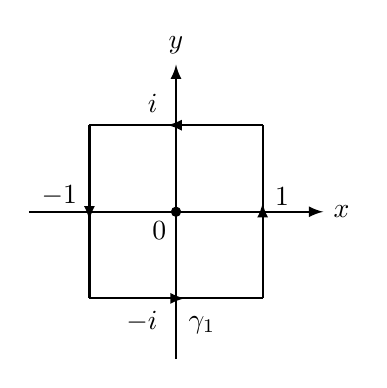
\begin{tikzpicture}[scale=1.1, >=latex]
    % Координатные оси
    \draw[->, thick] (-1.7, 0) -- (1.7, 0) node[right] {$x$};
    \draw[->, thick] (0, -1.7) -- (0, 1.7) node[above] {$y$};
    \node[below left] at (0, 0) {$0$};

    % Особая точка в нуле
    \filldraw (0,0) circle (1.5pt);

    % Стороны квадрата и стрелки обхода (против часовой стрелки)
    % 1) Нижняя сторона: gamma_1 (-1,-1) -> (1,-1)
    \draw[thick] (-1, -1) -- (1, -1);
    \draw[thick, ->] (-1, -1) -- (0.1, -1);
    \node[below] at (0.3, -1.1) {$\gamma_1$};

    % 2) Правая сторона: (1,-1) -> (1,1)
    \draw[thick] (1, -1) -- (1, 1);
    \draw[thick, ->] (1, -1) -- (1, 0.1);

    % 3) Верхняя сторона: (1,1) -> (-1,1)
    \draw[thick] (1, 1) -- (-1, 1);
    \draw[thick, ->] (1, 1) -- (-0.1, 1);

    % 4) Левая сторона: (-1,1) -> (-1,-1)
    \draw[thick] (-1, 1) -- (-1, -1);
    \draw[thick, ->] (-1, 1) -- (-1, -0.1);

    % Засечки координат
    \draw (-1, 2pt) -- (-1, -2pt) node[above left=1pt] {$-1$};
    \draw (1, 2pt) -- (1, -2pt) node[above right=1pt] {$1$};
    \draw (2pt, 1) -- (-2pt, 1) node[above left=1pt] {$i$};
    \draw (2pt, -1) -- (-2pt, -1) node[below left=1pt] {$-i$};
\end{tikzpicture}
\end{minipage}%
\hfill
\begin{minipage}[c]{0.61\textwidth}
\small
Рассмотрим сторону квадрата $\gamma_1$: $z(t) = t - i$, где $t \in [-1; 1]$, тогда $dz = dt$:
\[
\int_{\gamma_1} \frac{dz}{z} = \int_{-1}^{1} \frac{dt}{t - i} = \int_{-1}^{1} \frac{t + i}{t^2 + 1}
\,dt = \int_{-1}^{1} \frac{t\,dt}{t^2 + 1} + i \int_{-1}^{1} \frac{dt}{t^2 + 1}.
\]

Первый интеграл равен $0$ в силу нечётности подынтегральной функции, а второй:
\[
\int_{-1}^{1} \frac{dt}{t^2 + 1} = \operatorname{arctg}(1) - \operatorname{arctg}(-1) = 
\frac{\pi}{4} - \left(-\frac{\pi}{4}\right) = \frac{\pi}{2}.
\]
Откуда получаем $\displaystyle\int_{\gamma_1} \frac{dz}{z} = i\,\frac{\pi}{2}$.
\end{minipage}

\medskip\noindent
Для остальных сторон квадрата используем поворот: замена $z = iw$ (при которой $dz = i\,dw$ и 
$\frac{dz}{z} = \frac{dw}{w}$) последовательно переводит отрезки друг в друга с сохранением 
ориентации. Следовательно, интегралы по всем 4 сторонам равны между собой:
\[
\oint_{\partial K} \frac{dz}{z} = 4 \int_{\gamma_1} \frac{dz}{z} = 4 \cdot \frac{i\pi}{2} = 2\pi i.
\]
Делая замену $w = a + \varepsilon z$ ($\varepsilon > 0$), получаем для произвольного квадрата 
$K_\varepsilon(a)$ с центром в точке $a$:
\[
\oint_{\partial K_\varepsilon(a)} \frac{dw}{w - a} = \oint_{\partial K} 
\frac{\varepsilon\,dz}{\varepsilon z} = \oint_{\partial K} \frac{dz}{z} = 2\pi i.
\]
\end{example}


\Section{Первообразная}

\begin{definition}
    Функция \(F(z)\) называется \textit{первообразной} для регулярной в области \(G \subset \Co\) 
    \(f(z)\), если \(F'(z) = f(z)\) для любого \(z \in G\).
\end{definition}

\begin{statement}
    Пусть \(f(z)\) имеет первообразную \(F_1(z)\). Тогда \(\forall C \in \Co \rightarrow F_1 + C\)
    ~--- первообразная \(f(z)\) и если \(F_2\) также является первообразной \(f(z)\), то верно
    \(F_2(z) - F_1(z) = \text{const}\) в области \(G\).
\end{statement}

\begin{proof}
    Первая часть доказываемого утверждения очевидна из определения первообразной.

    Пусть \(F_2(z) - F_1(z) = F(z)\). Так как \(F_1'(z)=F_2'(z) = f(z)\), то \(F'(z) = 0\). 
    Для доказательства необходимо получить, что \(F(z) = \text{const}\). Пусть \(F(z) = 
    U(x, y) + iV(x, y)\). Из утверждения\ref{9:Koshi_Riman} \(F'(z) = U_x + iV_x = U_x - iU_y\). Так
    как \(F'(z) = 0\), то \(U_x = 0\) и \(U_y = 0\). Зафиксируем точки \((x_0, y_0), \, (x_{00}, 
    y_{00}) \in G\). Эти две точки можно отрезком кривой из \(G\). При этом он задаётся гладкой 
    функцией \(x = x(t), \, y = y(t), \, \alpha \le t \le \beta\). Для \(\Phi(t) = U(x(t), y(t))\) 
    имеем \(\Phi'(t) = U_x x' + U_y y' = 0\) на \([\alpha, \beta]\). Тогда \(U(x_0, y_0) = 
    \Phi(\alpha) = \Phi(\beta) = U(x_{00}, y_{00})\). Так как \(G\)~--- область, то в любых точках 
    \(U\) совпадает, а значит равна постоянной. Аналогично для \(V\). Тогда \(F = \text{const} \in 
    \Co\).
\end{proof}

\begin{statement} \label{12:int_kontur}
    \begin{enumerate}[wide=20pt, label=\arabic*., itemsep=0ex]
        \item Если непрерывная непрерывная на области \(G\) имеет в ней первообразную \(F(z)\), то
        \(\int\limits_\gamma f(z) dz = 0\) для любого КНД контура в \(G\).
        \item Если \(f(z)\) непрерывна на области \(G\) и \(\int\limits_\gamma f(z) dz = 0\) для
        любой простой замкнутой конечнозвенной ломаной в \(G\), то \(f\) имеет первообразную.
    \end{enumerate}
\end{statement}

\begin{proof}
    \begin{enumerate}[wide=5pt, label=\arabic*., itemsep=0ex]
        \item \(\Phi(t) = F(z(t))\), где \(F\)~--- первообразная \(f\); \(z = z(t)\), \(t \in 
        [\alpha, \beta]\)~--- параметризация \(\gamma\). \(\Phi'(t) = F'(z(t))z'(t) = f(z(t))
        z'(t)\). Пусть \(z_0 = z(\alpha), \, z_{00} = z(\beta)\), тогда \(F(z_{00}) - F(z_0) = 
        F(z(\beta)) - F(z(\alpha)) = \Phi(\beta) - \Phi(\alpha) = \int\limits_\alpha^\beta \Phi'(t)
        dt = \int\limits_\alpha^\beta f(z(t))z'(t)dt = \int\limits_\gamma f(z)dz\). Итак, если 
        непрерывная \(f\) имеет первообразную, то справедлива формула Ньютона-Лейбница:
        \(F(z_{00}) - f(z_0) = \int\limits_\gamma f(z)dz\), где \(\gamma\)~--- КНД кривая, 
        соединяющая \(z_0, \, z_{00}\).

        \item а). Из условий следует, что для любой замкнутой конечнозвенной ломаной (возможно, 
        непростой) будет выполняться \(\int\limits_\gamma f(z)dz = 0\), так как ломаная разобьётся
        на конечное число многоугольников, стороны которых будут представлять из себя контуры.

        б). Тогда верно, что \(\int\limits_{\gamma_1} f(z)dz = \int\limits_{\gamma_2} f(z)dz\) для 
        любых конечнозвенных ломаных соединяющих 2 точки \(z_0, \, z_{00}\). Зафиксируем точку
        \(z_0 \in G\). \(\forall \in G\) определим \(F(z) = \int\limits_{z_0}^{z} f(\zeta) d\zeta\)
        по \(\gamma \subset G\)~--- конечнозвенной ломаной, соединяющей \(z_0, z\). Докажем, что \(
        F'(z) = f(z)\). Зафиксируем \(\epsilon > 0\). Выберем \(\delta > 0\) такое, что \(\forall
        \Delta z \in B_\delta (0) \rightarrow |\rho(z+\Delta z) - \rho(z)| < \epsilon\). Теперь
        зафиксируем \(\Delta z \in \mathring{B}_\delta (0)\). Тогда \(|\dfrac{F(z+\Delta z - F(z))}
        {\Delta z} - f(z)| = |\dfrac{1}{\Delta z}(\int\limits_{z_0}^{z+\Delta z} f(z)dz - 
        \int\limits_{z_0}^{z}) - f(z)| = |\dfrac{1}{\Delta z}(\int\limits_{z}^{z+\Delta z} (f(w) - 
        f(z))dw)| \le \epsilon\). В силу произвольности \(\epsilon\) получаем определение того, что
        \(f(z)\) производная \(F(z)\).
    \end{enumerate}
\end{proof}

\begin{example}
    \(f(z) = \dfrac{1}{z-a}\) не имеет первообразной в \(\Co \setminus {a}\), так как \(
    \int\limits_\gamma \dfrac{1}{z-a} = 2\pi i \ne 0\) в соответствии с примером 
    \ref{11:int_square}.
\end{example}


\Section{Степенные ряды}

В этом параграфе за \((*)\) будем принимать ряд \(\sum\limits_{n=0}^\infty{c_n(z-z_0)^n}\).

\begin{theorem}
    Если ряд \((*)\) сходится при некотором \(\tilde{z} < z_0\), то
    \begin{enumerate}[wide=20pt, label=\arabic*., itemsep=0ex]
        \item он абсолютно сходится для любого \(z \colon \, |z-z_0|<|\tilde{z} - z_0|\),
        \item он равномерно сходится в любом круге \(|z-z_0| \le r < |\tilde{z} - z_0|\).
    \end{enumerate}
\end{theorem}

\begin{corollary}
    Если ряд \((*)\) расходится в точке \(\tilde{z} \ne z_0\), то он расходится для любого \(z 
    \colon \, |z-z_0| > |\tilde{z}-z_0|\).
\end{corollary}

\begin{corollary}
    Если ряд \((*)\) сходится в круге \(|z-z_0| < R\), то он сходится абсолютно.
\end{corollary}

\begin{statement}
    Пусть ряд \(\sum\limits_{n=0}^\infty{c_n z^n}\) (обозначим за \((1)\)) сходится в круге \(|z| <
    R\) (обозначим за \(K\)) к сумме \(S(z)\). Тогда:
    \begin{enumerate}[wide=20pt, label=\arabic*., itemsep=0ex]
        \item ряд \(\sum\limits_{n=0}^\infty{n c_n z^{n-1}}\) (обозначим за \((2)\)) сходится в том
        же круге к некоторой сумме \(S_1(z)\),
        \item \(S'(z) \equiv S_1(z)\) в \(K\).
    \end{enumerate}
\end{statement}

\begin{proof}
    \begin{enumerate}[wide=5pt, label=\arabic*., itemsep=0ex]
        \item Зафиксируем \(z \in K\) и докажем сходимость ряда \((2)\) в этой точке. Пусть 
        \(|\tilde{z}| \in K\), тогда \(|n c_n z^{n-1}| \le |c_n \tilde{z}^n|\) для всех достаточно 
        больших \(n\). Так как ряд \((1)\) сходится, то ряд \((2)\) также сходится.
        \item \(S_1(z) \in C(K)\). Пусть \(\gamma\)~--- КНД контур в \(K\). Носитель \(\gamma\)~---
        компакт, поэтому ряд \((2)\) сходится равномерно на \(\gamma\). \(\int\limits_\gamma S_1(z)
        dz = \sum\limits_{n = 1}^\infty \int\limits_\gamma n c_n z^{n-1} dz = 0\), так как при 
        каждом \(n\) найдётся производная, то есть все члены суммы равны нулю. В силу утверждения
        \ref{12:int_kontur} \(S_1(z)\) имеет первообразную в \(K\) и одна из них равна \(\hat{S}(z)
        = \int\limits_0^z{S_1(\zeta) d\zeta} = \sum\limits_{n=1}^\infty c_n z^n\). Отличие ряда 
        \((1)\) и полученной первообразной~--- постоянная, а значит ряд \((1)\) также первообразная
        ряда \((2)\).
    \end{enumerate}
\end{proof}

\begin{corollary}
    \(S(z)\) бесконечно непрерывно дифференцируема в круге \(K\). То есть \(\sum\limits_{n=0}^\infty
    {c_n z^n}\)~--- ряд Тейлора своей суммы.
\end{corollary}


\Section{Интеграл Коши}

Пусть \(\gamma\)~--- КНД кривая, \(f \in C(\gamma)\). Для \(z \notin \gamma\) определим интеграл
Коши: \[F(z) = \dfrac{1}{2 \pi i} \int\limits_\gamma \dfrac{f(\zeta)}{\zeta - z} d\zeta \tag{1}\].

\begin{statement}
    Если \(B_R (z_0) \cap \gamma = \emptyset\), то \(f(z)\) представляется степенным рядом \(F(z) =
    \sum\limits_{n=0}^\infty{c_n(z-z_0)^n}\), где \(c_n = \dfrac{1}{2 \pi i} \int\limits_\gamma
    \dfrac{f(\zeta) d\zeta}{(\zeta - z_0)^{n+1}}\).
\end{statement}